\documentclass[a4paper,11pt]{article}

\usepackage[T1]{fontenc}
\usepackage{lmodern}
\usepackage[margin=2.5cm]{geometry}
\usepackage{graphicx}
\usepackage{float}
\usepackage{xcolor}
\usepackage{booktabs}
\usepackage{tabularx}
\usepackage{enumitem}
\usepackage{amsmath}
\usepackage{lastpage}
\usepackage{fancyhdr}
\usepackage{tikz}
\usetikzlibrary{positioning,arrows.meta,fit,backgrounds}
\usepackage[colorlinks=true,urlcolor=bsgreen,linkcolor=black]{hyperref}

\definecolor{bsgreen}{HTML}{1E7D4F}
\definecolor{bslight}{HTML}{E8F3EC}
\definecolor{bsorange}{HTML}{E8693F}
\definecolor{bsgrey}{HTML}{5A6670}

\pagestyle{fancy}
\fancyhf{}
\fancyhead[L]{\small\color{bsgrey} BesinSkor: Technical Overview}
\fancyhead[R]{\small\color{bsgrey} G\"orkem \"Ozbek}
\fancyfoot[C]{\small\color{bsgrey} \thepage\ / \pageref{LastPage}}
\renewcommand{\headrulewidth}{0.3pt}

\setlength{\parindent}{0pt}
\setlength{\parskip}{0.6em}
\setlist{itemsep=0.15em, topsep=0.3em}
\newcommand{\code}[1]{\texttt{#1}}

\begin{document}

%================ TITLE ================
\thispagestyle{empty}
\begin{center}
\vspace*{2.2cm}

\includegraphics[width=2.6cm]{../screenshots/icon.png}\\[1em]
{\fontsize{34}{40}\selectfont\bfseries\color{bsgreen} BesinSkor}\\[0.6em]
{\Large Scan a food product, understand what you eat}\\[2.2em]
{\large Technical overview of a published mobile application}\\[0.4em]
{\color{bsgrey} iOS (App Store) \textperiodcentered{} Android (Google Play, closed testing) \textperiodcentered{} \href{https://besinskor.com}{besinskor.com}}\\[3em]
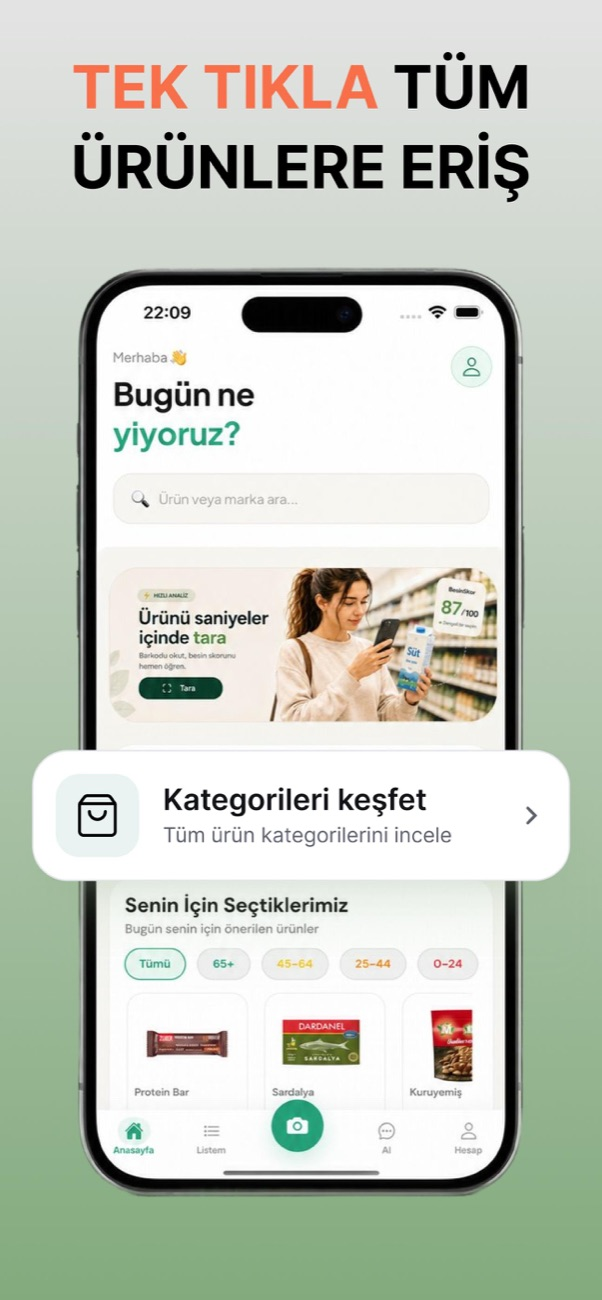
\includegraphics[height=7.2cm]{../screenshots/02-home.jpg}\hspace{0.4cm}
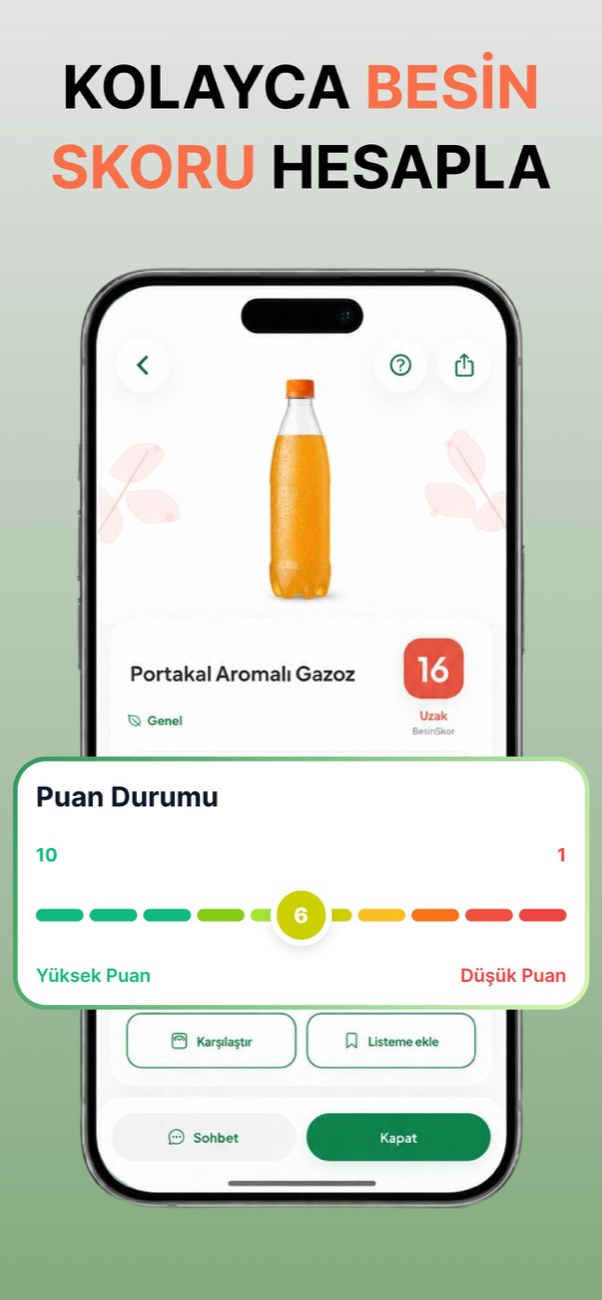
\includegraphics[height=7.2cm]{../screenshots/03-product-score.jpg}\hspace{0.4cm}
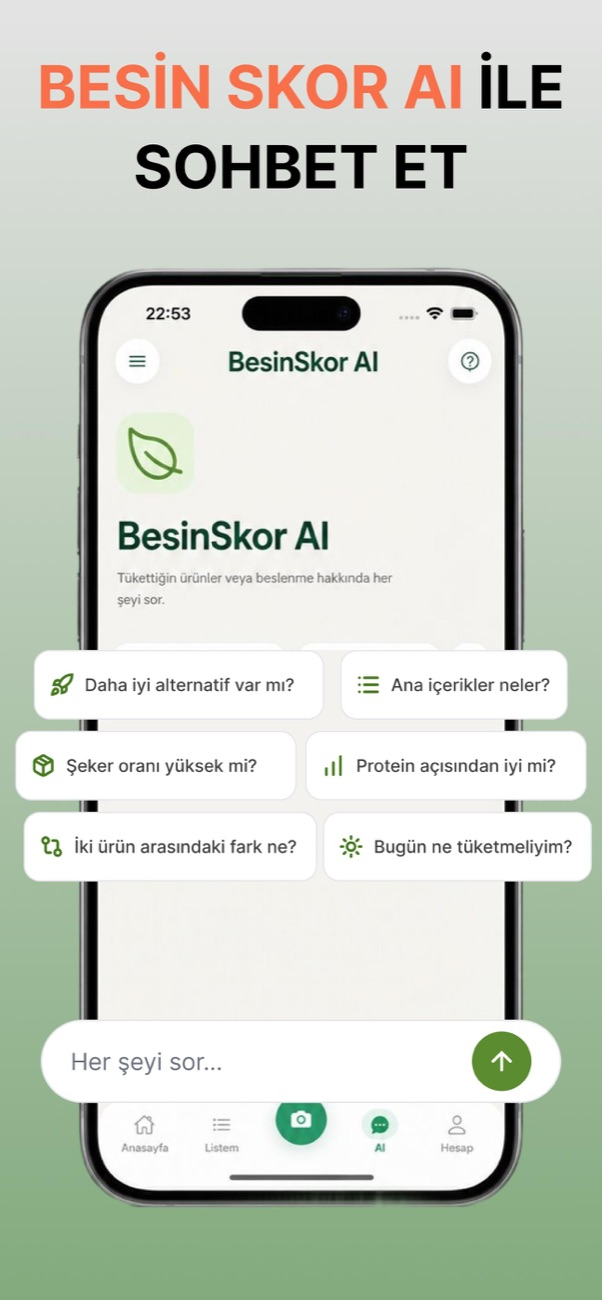
\includegraphics[height=7.2cm]{../screenshots/05-ai-assistant.jpg}\\[3em]
{\large\bfseries G\"orkem \"Ozbek}\\[0.3em]
{\color{bsgrey} Galatasaray University \textperiodcentered{} 2026}
\end{center}
\newpage

\tableofcontents
\newpage

%================ 1 ================
\section{Overview}

BesinSkor is a mobile application that helps people in T\"urkiye understand the nutritional quality of packaged food. The user scans a product's barcode, and the app shows a simple health score from \textbf{A} (best) to \textbf{E}, a score out of 100, and the product's level of processing. An AI assistant then answers questions about the product or about the user's diet.

I designed, built and published the whole product: the scoring algorithm, the mobile app for iOS and Android, the website, the backend and database, the AI integration, the subscriptions, and the release on the stores.

\begin{center}
\begin{tabularx}{0.95\linewidth}{@{}lX@{}}
\toprule
\textbf{Platforms} & iOS (App Store, since June 2026), Android (Google Play, closed testing), web \\
\textbf{Store category} & Health \& Fitness \\
\textbf{App Store rating} & 5.0 / 5 \\
\textbf{Current version} & 1.0.6 (November 2026) \\
\textbf{Main language} & Turkish (English and French in progress) \\
\textbf{Business model} & Free app with a \emph{BesinSkor Plus} subscription \\
\bottomrule
\end{tabularx}
\end{center}

\begin{center}
\fbox{\parbox{0.9\linewidth}{\small BesinSkor is a commercial product, so its source code is private. This document describes its design and the technical choices behind it, without publishing code or credentials.}}
\end{center}

%================ 2 ================
\section{Problem and Users}

Nutrition labels list many numbers (energy, sugars, saturated fat, salt, fibre, protein) that are hard to compare quickly in a supermarket. In T\"urkiye, most packaged products have no simple front-of-pack score. As a result, it is difficult to know whether a product is a healthy choice, or which of two similar products is better.

BesinSkor targets everyday shoppers, people following a diet or a health goal, and parents choosing food for their children. The design goals were:
\begin{itemize}
  \item \textbf{Fast}: a result in a few seconds, directly in the shop;
  \item \textbf{Simple}: one letter and one colour that anyone understands;
  \item \textbf{Explainable}: the user can always see \emph{why} a product got its score;
  \item \textbf{Local}: Turkish products, Turkish language, Turkish categories.
\end{itemize}

%================ 3 ================
\section{Features}

\begin{figure}[H]
\centering
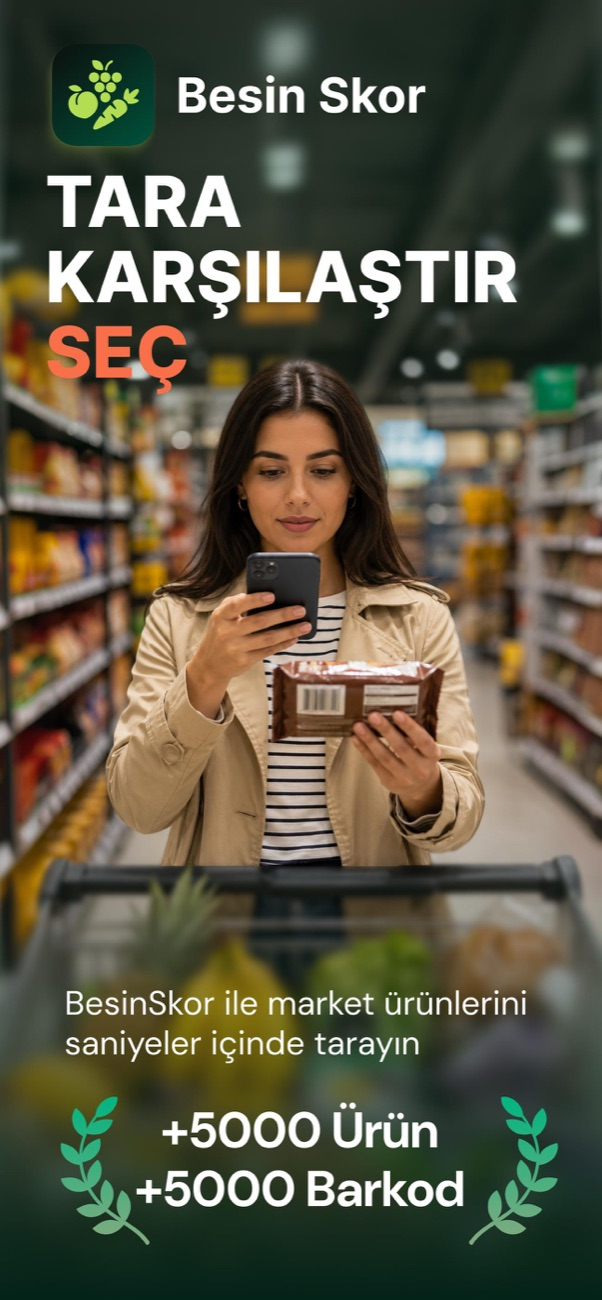
\includegraphics[height=6.4cm]{../screenshots/01-scan.jpg}\hfill
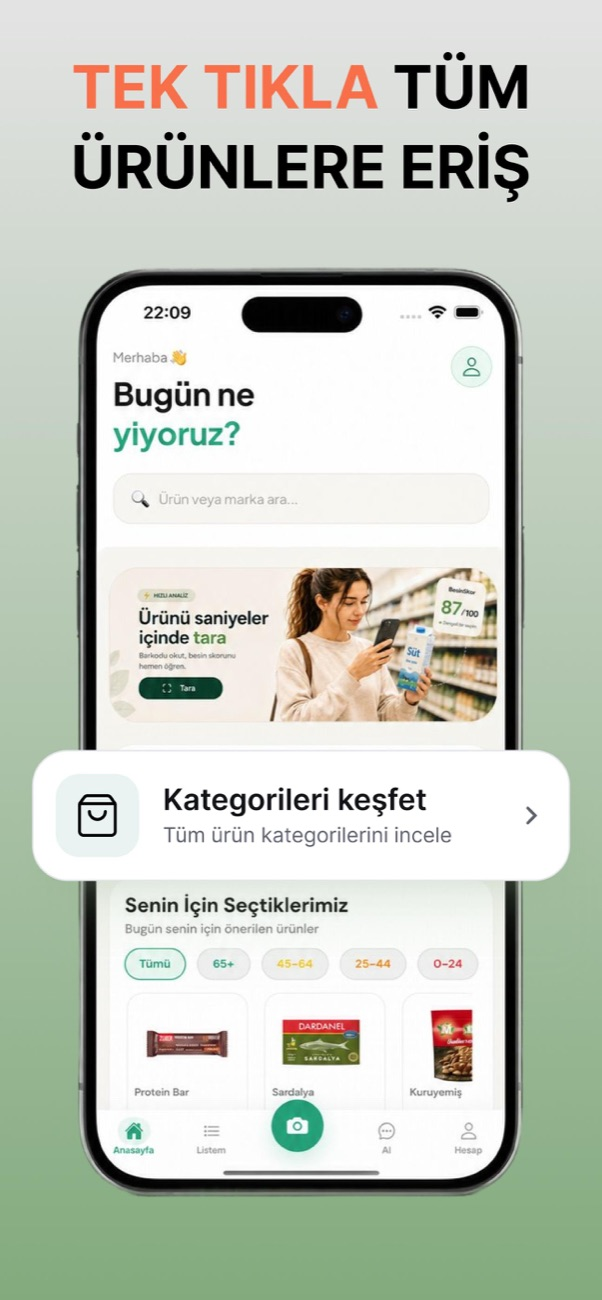
\includegraphics[height=6.4cm]{../screenshots/02-home.jpg}\hfill
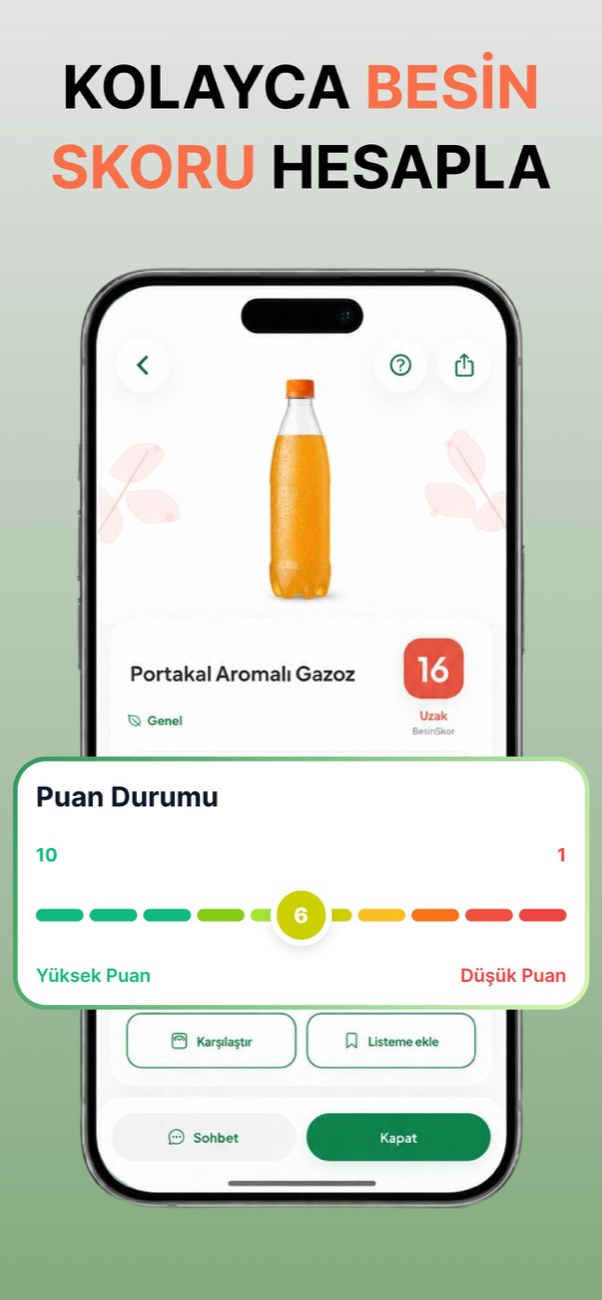
\includegraphics[height=6.4cm]{../screenshots/03-product-score.jpg}\hfill
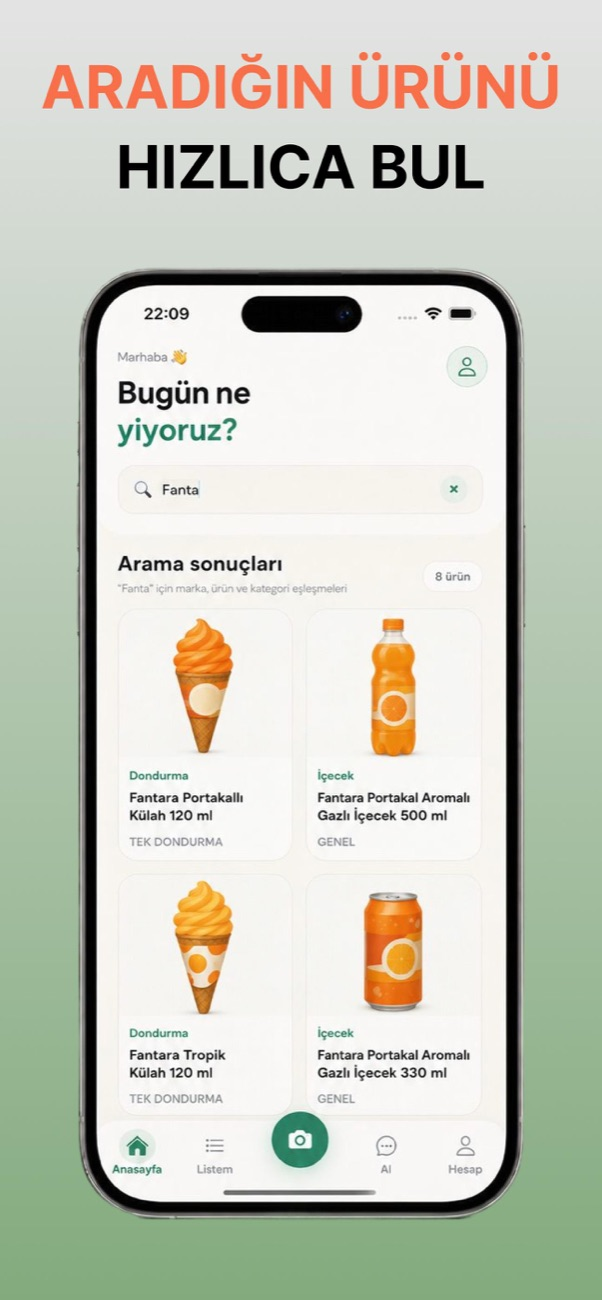
\includegraphics[height=6.4cm]{../screenshots/04-search.jpg}\hfill
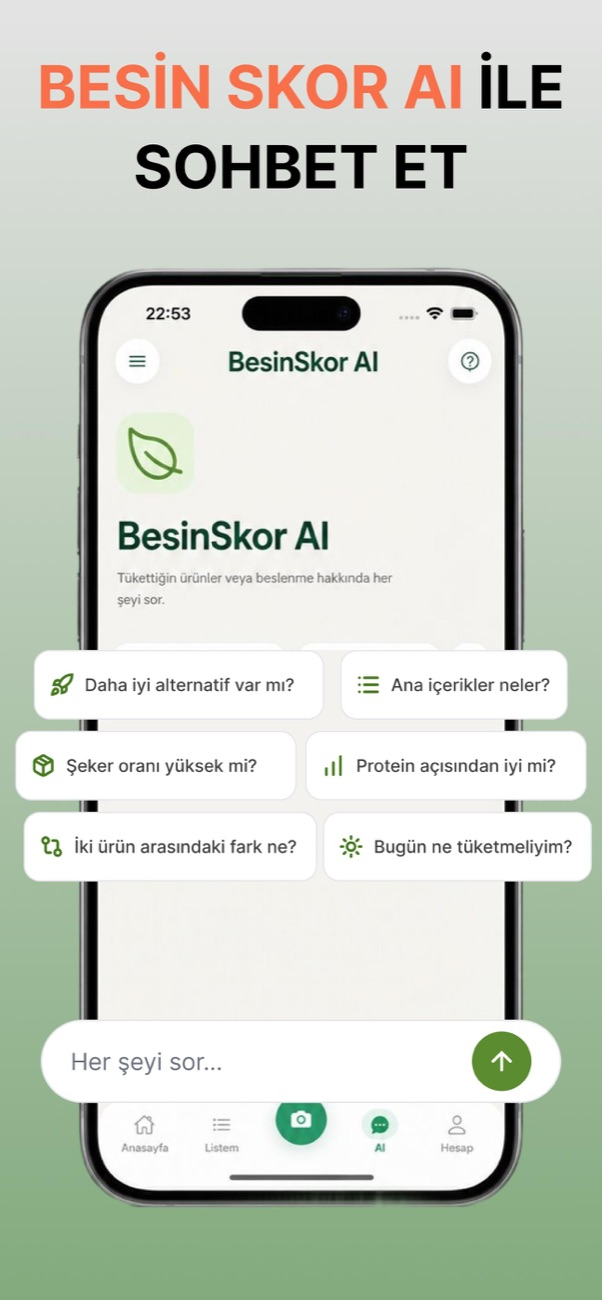
\includegraphics[height=6.4cm]{../screenshots/05-ai-assistant.jpg}
\caption{App Store screenshots: scanning, home screen, product score, search and AI assistant.}
\end{figure}

\begin{tabularx}{\linewidth}{@{}lX@{}}
\toprule
\textbf{Feature} & \textbf{Description} \\
\midrule
Barcode scanner & Camera scan with instant lookup in the BesinSkor database, and a fallback to Open Food Facts for international products. \\
Health score & Letter A--E, score out of 100, colour scale, and the NOVA processing group. \\
Search and categories & Search by product or brand name, browse by category, filter by score. \\
AI assistant & Chat about a product (\emph{``Why this score?'', ``Is there a better alternative?''}) or about the user's diet. \\
Compare & Two products side by side. \\
My List & Daily list of consumed products, with statistics and streaks. \\
Nutrition profile & Gender, age, goal, height and weight, used to personalise advice. \\
Community products & Users submit a missing barcode with photos; an administrator approves or rejects it. \\
BesinSkor Plus & Monthly and yearly subscriptions with a 7-day free trial. \\
Notifications & Reminders and usage-limit notifications. \\
\bottomrule
\end{tabularx}

%================ 4 ================
\section{Architecture}

\begin{figure}[H]
\centering
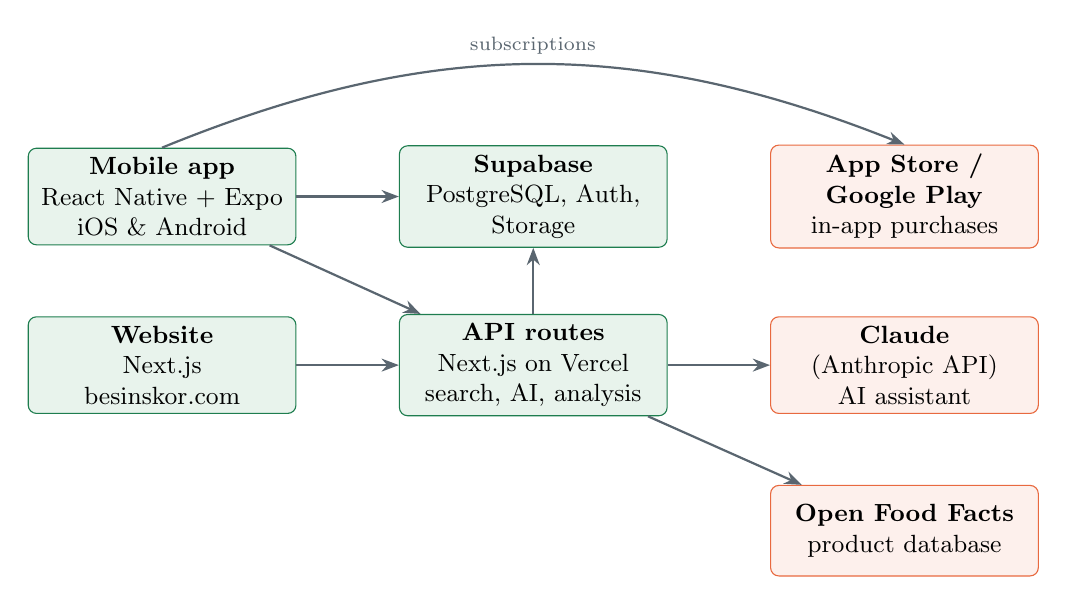
\begin{tikzpicture}[
  node distance=0.9cm and 1.3cm,
  box/.style={draw=bsgreen, fill=bslight, rounded corners=3pt, align=center, minimum width=3.4cm, minimum height=1.15cm, font=\small},
  ext/.style={draw=bsorange, fill=bsorange!10, rounded corners=3pt, align=center, minimum width=3.4cm, minimum height=1.15cm, font=\small},
  arr/.style={-{Stealth[length=2.2mm]}, thick, color=bsgrey}
]
\node[box] (app) {\textbf{Mobile app}\\React Native + Expo\\iOS \& Android};
\node[box, below=of app] (web) {\textbf{Website}\\Next.js\\besinskor.com};
\node[box, right=of app] (db) {\textbf{Supabase}\\PostgreSQL, Auth,\\Storage};
\node[box, right=of web] (api) {\textbf{API routes}\\Next.js on Vercel\\search, AI, analysis};
\node[ext, right=of db] (store) {\textbf{App Store /}\\\textbf{Google Play}\\in-app purchases};
\node[ext, right=of api] (ai) {\textbf{Claude}\\(Anthropic API)\\AI assistant};
\node[ext, below=of ai] (off) {\textbf{Open Food Facts}\\product database};

\draw[arr] (app) -- (db);
\draw[arr] (app) -- (api);
\draw[arr] (web) -- (api);
\draw[arr] (api) -- (db);
\draw[arr] (api) -- (ai);
\draw[arr] (api) -- (off);
\draw[arr] (app.north) to[bend left=22] node[above, font=\scriptsize]{subscriptions} (store.north);
\end{tikzpicture}
\caption{High-level architecture. Green: my components. Orange: external services.}
\end{figure}

\textbf{One backend, two clients.} The mobile app and the website share the same Supabase project (PostgreSQL database, authentication and file storage) and the same server-side API routes. The app talks to Supabase directly for user data (lists, favourites, profile), and goes through the API for anything that needs a secret key, such as the AI assistant.

\textbf{Main data model.} The database holds products and their nutrition values, user favourites and history, AI conversations, product reviews, community submissions, subscriptions, nutrition profiles and analytics events.

\textbf{Mobile stack.} React Native 0.81 with Expo SDK 54 and TypeScript, React Navigation (tabs and stacks), \code{expo-camera} for scanning, \code{expo-iap} for purchases and \code{expo-notifications}. Builds and store submissions go through EAS Build and EAS Submit.

\textbf{Web stack.} Next.js 16 (App Router), React 19, TypeScript and Tailwind CSS, deployed on Vercel. Product pages are public and indexable, which brings visitors from search engines. The score itself is only shown in the app, so the website also works as a funnel to the app stores.

%================ 5 ================
\section{The Scoring Algorithm}

The score is computed by a \textbf{deterministic algorithm}, not by the AI. This keeps it reproducible, explainable and cheap to compute.

\subsection*{Basis: Nutri-Score 2023}
The algorithm follows the revised Nutri-Score (2023), the European front-of-pack label. Its thresholds were checked against the open-source implementation of Open Food Facts on reference products. For each product:
\begin{itemize}
  \item \textbf{negative points} come from energy, sugars, saturated fat and salt (and sweeteners for drinks);
  \item \textbf{positive points} come from fibre, protein, and fruits, vegetables and legumes;
  \item the raw score is $\text{negative points} - \text{positive points}$: lower is better.
\end{itemize}

\subsection*{Food categories}
The thresholds are different for three families, detected from the product's category:
\begin{itemize}
  \item \textbf{general foods};
  \item \textbf{beverages}, with stricter sugar and energy scales, a penalty for sweeteners, and water always rated best;
  \item \textbf{fats, oils, nuts and seeds}, where saturated fat is measured as a share of total fat.
\end{itemize}
Special rules from the specification are applied to cheese and red meat.

\subsection*{From raw score to BesinSkor}
The raw score is converted to a letter (A--E) with the category's thresholds, and to a \textbf{score out of 100} (0 = worst, 100 = best) that is easier to read and to compare. The \textbf{NOVA group} (1 = unprocessed to 4 = ultra-processed) is shown \emph{next to} the score and never mixed into it, so the two pieces of information stay clear.

%================ 6 ================
\section{AI Assistant}

The assistant uses Claude through the Anthropic API, called only from the server so that the API key is never shipped inside the app.

\begin{itemize}
  \item \textbf{Grounded answers}: the product's name, category, nutrition values and score are sent to the model as context, so it explains the real data instead of guessing.
  \item \textbf{Explain, don't decide}: the model never computes the score. It explains it, suggests alternatives and answers diet questions.
  \item \textbf{Product research}: when the user asks about a product that is not selected, the server first searches Open Food Facts by name and gives the result to the model.
  \item \textbf{Short history}: only the last messages are sent, which keeps answers relevant and costs low.
  \item \textbf{Cost control}: free users get a small number of messages per day, Plus users a larger quota. The limit is enforced on the server by a database function, not only in the app.
\end{itemize}

%================ 7 ================
\section{Data}

\begin{itemize}
  \item \textbf{Own product database} of Turkish products, with nutrition values, categories, images and barcodes.
  \item \textbf{Open Food Facts} as a fallback for international products; alcoholic and empty entries are filtered out.
  \item \textbf{Community submissions}: when a barcode is unknown, the user can send it with photos of the package. Each submission is reviewed by an administrator before it is added.
  \item \textbf{Data quality scripts} (Node.js) to audit and enrich the catalogue: missing values, wrong categories, duplicated barcodes.
\end{itemize}

%================ 8 ================
\section{Security and Privacy}

\begin{itemize}
  \item \textbf{Row-level security} in PostgreSQL: each user can only read and write their own lists, profile and conversations.
  \item \textbf{Secrets stay on the server}: the AI key and the database service key are only used in server-side API routes.
  \item \textbf{Server-side quotas} for AI requests, so the limits cannot be bypassed by calling the API directly.
  \item \textbf{Safe moderation actions}: links sent to the administrator open a confirmation page, and the action itself requires a POST request, so a link preview or crawler cannot approve or delete content by accident.
  \item \textbf{Input validation} on the analytics endpoint (allowed event names, size limits).
  \item \textbf{Account deletion} removes the user's data, including submissions and analytics events.
\end{itemize}

%================ 9 ================
\section{Business Model}

The app is free to download. \textbf{BesinSkor Plus} unlocks more AI messages and extra features, with monthly and yearly plans and a 7-day free trial. Purchases go through Apple and Google in-app purchases, and prices are shown in each user's local currency by the stores.

%================ 10 ================
\section{Release Process}

\begin{itemize}
  \item \textbf{Builds}: EAS Build for iOS and Android, EAS Submit to App Store Connect.
  \item \textbf{App Review}: one version was rejected under Apple's subscription guideline because the App Store description had no link to the Terms of Use. I added the Terms of Use and Privacy Policy links, and the next version was approved.
  \item \textbf{Google Play}: new developer accounts must run a closed test with real testers for 14 days before a public release. The app is currently in this phase.
  \item \textbf{Iterating with users}: bug reports from users (for example a blank-screen issue on the account tab) were fixed and shipped in the next version.
\end{itemize}

%================ 11 ================
\section{What I Learned}

\begin{itemize}
  \item Taking a product from an idea to a public release, including store rules, reviews and rejections.
  \item Building one codebase for two mobile platforms, and sharing a backend between an app and a website.
  \item Designing a relational database with authentication, storage and row-level security.
  \item Integrating a large language model in a product: context, cost, quotas, and keeping important decisions in deterministic code.
  \item Implementing subscriptions and free trials on both Apple and Google.
  \item Working with real users: feedback, bug reports, community content and moderation.
\end{itemize}

\section{Next Steps}
\begin{itemize}
  \item Public release on Google Play.
  \item English and French versions of the app (translation done, release in progress).
  \item Server-side verification of subscriptions with the App Store and Google Play APIs.
  \item More products and more categories in the database.
\end{itemize}

\end{document}
